% A calendar of circles
% Author: Till Tantau (The PGF manual),
%   and Stefan Kottwitz (Modifications such as shaded circles and color)
\documentclass[tikz,dvisvgm]{standalone}

\usetikzlibrary{calendar,shadings}
\renewcommand*{\familydefault}{\sfdefault}
\colorlet{winter}{blue}
\colorlet{spring}{green!60!black}
\colorlet{summer}{orange}
\colorlet{fall}{red}
% A counter, since TikZ is not clever enough (yet) to handle
% arbitrary angle systems.
\newcount\mycount
\begin{document}
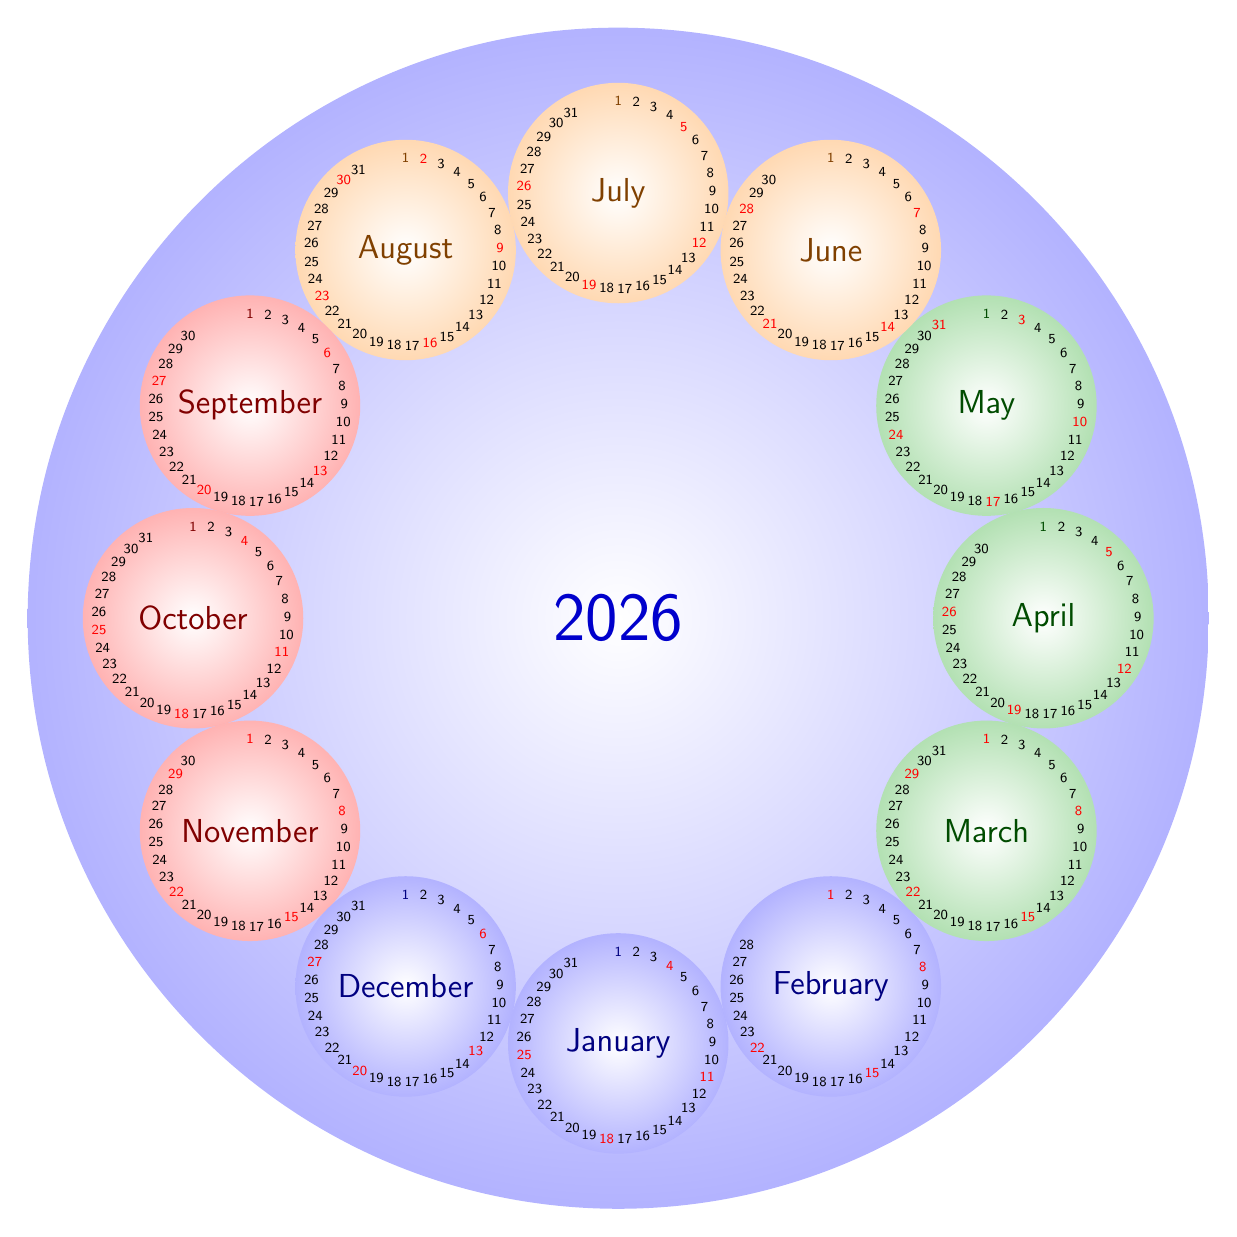
\begin{tikzpicture}[transform shape,
  every day/.style={anchor=mid,font=\tiny}]
  \node[circle,shading=radial,outer color=blue!30,inner color=white,
    minimum width=15cm] {\textcolor{blue!80!black}{\Huge\the\year}};
  \foreach \month/\monthcolor in
    {1/winter,2/winter,3/spring,4/spring,5/spring,6/summer,
    7/summer,8/summer,9/fall,10/fall,11/fall,12/winter} {
      % Computer angle:
      \mycount=\month
      \advance\mycount by -1
      \multiply\mycount by 30
      \advance\mycount by -90
      \shadedraw[shading=radial,outer color=\monthcolor!30,middle color=white,
        inner color=white,draw=none] (\the\mycount:5.4cm) circle(1.4cm);
      % The actual calendar
      \calendar at (\the\mycount:5.4cm) [
          dates=\the\year-\month-01 to \the\year-\month-last]
      if (day of month=1) {\large\color{\monthcolor!50!black}\tikzmonthcode}
      if (Sunday) [red]
      if (all) {
      % Again, compute angle
      \mycount=1
      \advance\mycount by -\pgfcalendarcurrentday
      \multiply\mycount by 11
      \advance\mycount by 90
      \pgftransformshift{\pgfpointpolar{\mycount}{1.2cm}}};}
\end{tikzpicture}
\end{document}